\documentclass{article}
\usepackage[T1]{fontenc}
\usepackage[utf8]{inputenc}

\usepackage{lmodern}
\usepackage{verbatim} 
\usepackage{eurosym}
\usepackage[english]{babel}
\usepackage{graphicx}
\usepackage{url}
\usepackage{subcaption}
\usepackage{caption}
\usepackage{enumerate}
\usepackage{float}

\usepackage[titletoc,title]{appendix}
\usepackage{amsmath}
\usepackage{booktabs}
\usepackage{wrapfig}

\renewcommand{\familydefault}{\sfdefault}
\bibliographystyle{plain}

\title{\textbf{Bachelor assignment proposal}}
  
\author{Rob Rikken}
\date{\today}

\begin{document}

\maketitle
\newpage
\tableofcontents
\newpage
\listoffigures
 \newpage
\listoftables
\newpage

\section{Introduction}
The developments in remote sensing and data gathering, has led to an abundance of data.
Satellite technology advancement in the recent decades has led to higher quality data of the earth.
The satellites now in orbit can identify the car you are driving, what color drink you are drinking, how high your house is.
For every half by half meter of the Netherlands, there is a height map entry.
Technologies like this are coinciding with a move to open data.
So there are now many different forms, types and precision's of data.

Waterboards, Rijkswaterstaat and private parties are all interested in using these types of data, but no standard has been set.
Parties believe the data can be useful, but don't know how to use it, yet. In this landscape, Deltares, Rijkswaterstaat and the waterboards of the Netherlands are working together on unifying the data that they gather into one system.
The first part of the workflow is ready. 

Waterboards can add their data to the database, and then it is provided to the general public via a data view portal. The data from the waterboards is already checked for the correct units with schemata. In these schemata units are checked but not consistency. The first few steps of integrating the data of waterboards into the NHI

\begin{figure}[h]
    \centering
    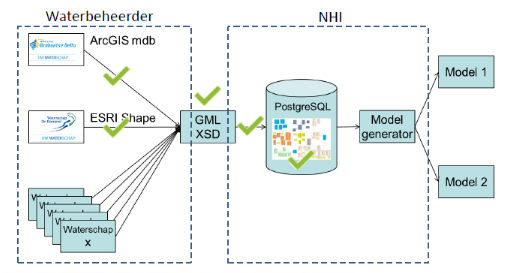
\includegraphics[width=\textwidth]{figures/database_nhi_flowchart.png}
    \caption{Waterboard data to NHI database.\cite{Kroon2016Overzicht}}
    \label{fig:nhi_data_cross_section}
\end{figure}

\begin{figure}[h]
    \centering
    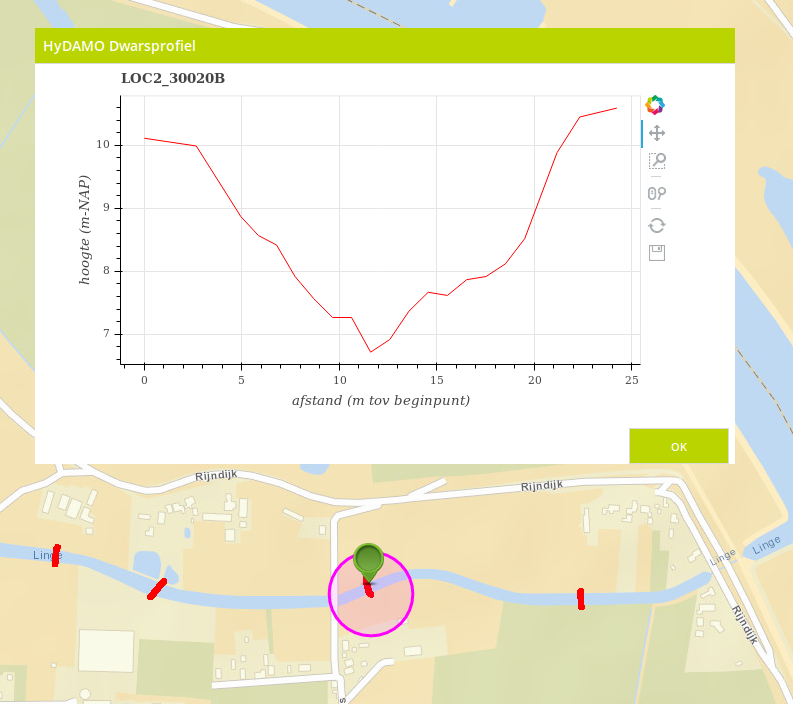
\includegraphics[width=\textwidth]{figures/cross_section_example.png}
    \caption{Cross section example from NHI data.\cite{NHI2019NHIPortaal}}
    \label{fig:nhi_data_cross_section}
\end{figure}

In the Netherlands, measurements of all types of characteristics of water have a long history. 
This means that satellites do not have the added value they might have in different countries. 
The value of the quality of the measurements in the Netherlands can however, be in the validation of the satellite measurements.
Advances in satellite bathymetry for instance, can be validated with the extensive measurements of all the waterways in the Netherlands.

Using all this data in the countrywide hydraulic model (Landelijk Hydrologisch Model, LHM), has not been easy. 
Every waterboard, Rijkswaterstaat and other governmental and private parties, have different ways of storing the data. 
They all want to cooperate together, but because there are different practises making this a reality has taken some effort.

One way of making sure the data has the same types, is using XSD, a way of making sure XML files are using the same standard\cite{XSDStandaardisatie}.

\section{Research design}

\subsection{Theory}
\subsection{Aim of the research}
\subsection{Research questions}
\subsubsection{Data}
For the analysis if the cross sections have errors in them, two data sources are used.
The AHN2 map of the Netherlands and the cross sections, provided by the waterboards to the NHI.
The AHN map has data for the whole of the Netherlands in a resolution of 0,5 by 0,5 meters.
Height maps for the waterways are not available, but the embankments seem to be all there.
These might have an overlap between the cross section, so could be used to check for errors.
In the data portal of the NHI, the AHN2 map is already available and the cross sections of a few waterboards are available.
For the purpose of this research, the cross sections are detailed enough, they are represented in meters above NAP, just like the AHN map.
As the research focuses on the ability to detect errors, more then one board is can be used to check differences in quality of the data.

\subsection{Methods}
\section{Planning}
\subsection{Activities}
\subsection{Researching}
\subsection{Writing}
\newpage
\bibliography{references}
\end{document}